%%-------------------------------------------------------------------------------------------------
%%                           Template Notes:
%% Make sure to have all template files from klmweb/revisions/templates/JJH_Beamer before using
%% this file. Also please read the Beamer Reference document for typists if you have any questions
%% on the usage of this template.
% -------------------------------------------------------------------------------------------------
\documentclass[static]{JJH-Beamer}

%% -- Extra Packages (Place Packages here if they are not included in the default template)--------

\usepackage{booktabs}
\usepackage{soul}
\usepackage{tabularx}
\usepackage{graphicx}
\usepackage{colortbl}
\usepackage[para]{threeparttable}
\usepackage{epstopdf}
\usepackage{subfig}
\usepackage{bbding}
\usepackage{appendixnumberbeamer}

%% ------ Extra Preamble Definitions (Place any other extra preamble stuff here) ------------------

\newcommand{\mr}{\multirow}
\newcommand{\mc}{\multicolumn}
\newcolumntype{L}[1]{>{\raggedright\let\newline\\\arraybackslash\hspace{0pt}}m{#1}}
\newcolumntype{C}[1]{>{\centering\let\newline\\\arraybackslash\hspace{0pt}}m{#1}}
\newcolumntype{R}[1]{>{\raggedleft\let\newline\\\arraybackslash\hspace{0pt}}m{#1}}

\newcommand{\backupbegin}{
   \newcounter{finalframe}
   \setcounter{finalframe}{\value{framenumber}}
}
\newcommand{\backupend}{
   \setcounter{framenumber}{\value{finalframe}}
}

\newcommand*\leftright[2]{%
  \leavevmode
  \rlap{#1}%
  \hspace{0.5\linewidth}%
  #2}

% ------------ Title, author, date (ALWAYS UPDATE THESE THINGS) -----------------------------------

\def \thetitle {ABC and CARE: Some Clarifications} % Full title goes here

\def \theshorttitle {Analyzing Early Childhood Education} %Short title goes here

\def \theauthor {Jorge Luis Garc\'{i}a, James J. Heckman, Andr\'{e}s Hojman,\\ Duncan Ermini Leaf, Mar\'{i}a Jos\'{e} Prados, \\ Joshua Shea, Jake Torcasso} % Author name(s) go here

\def \theshortauthor {Garc\'{i}a et al.} % Short author name(s) go here; should fit on this one line.

\def \thedate {} % Date and venue information

\def \eventnotes {\noindent
\textbf{Date:}  \\
\textbf{Event Title:}  \\
\textbf{Host:}  \\
\textbf{Location:} \\
\textbf{Format:}  \\
\textbf{Length:} \\
\textbf{Audience Background:} 
} % Other event info, to appear on the front of the private notes

% -------------------------------------------------------------------------------------------------

\begin{document}
\renewcommand*{\inserttotalframenumber}{\pageref{lastframe}}
\mode<all>{\theTitlePages} % Macro to insert both title pages DO NOT REMOVE!

%%
%% ------------------------- Content starts here --------------------------------------------------
%%

%% ---------------------------------------------------------------------------

\begin{frame}
\frametitle{Plan for Presentation}
\begin{enumerate}
	\item Control substitution: providing participants by sex
	\item Treatment effects before control substitution onsets
	\item Compare ``old'', ``Tuesday's'', and ``current'  estimates
		\begin{itemize}
				\item Updates to crime in CARE, account for deaths 
		\end{itemize}
	\item Show empirical distributions of IRRs and BCs of ``current'' estimates
	\item Show new results: baseline, trimming, no controls
\end{enumerate}
\end{frame}

%% ---------------------------------------------------------------------------

\begin{frame}
\frametitle{Control-group Substitution}\label{substitution}
\begin{figure}
\caption{Months in Alternative Preschools (Control Group)}
	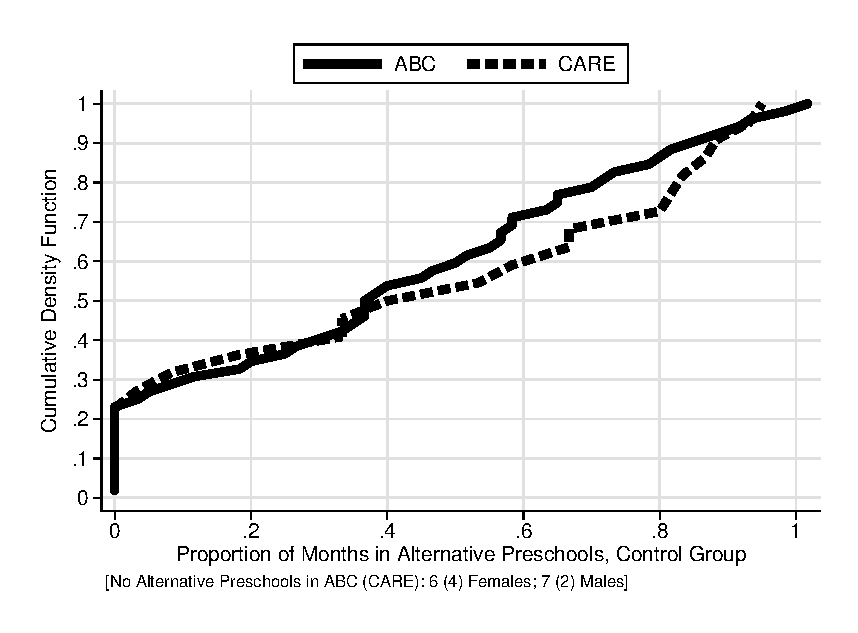
\includegraphics[width=20em]{output/abccare_controlcontamination.eps}
\end{figure}
\hyperlink{abc_subsidized}{\beamergotobutton{Proportion Subsidized, ABC}}
\hyperlink{care_subsidized}{\beamergotobutton{Proportion Subsidized, CARE}}
\end{frame}

%% ---------------------------------------------------------------------------

\begin{frame}
\frametitle{Alternative Preschools Take-up, ABC}\label{abc_subsidized}
\begin{figure}
\caption{Average Months in Control Substitution, ABC}
	\includegraphics[width=18em]{output/blackwhite_CCnumber}
\end{figure}
\hyperlink{substitution}{\beamerreturnbutton{Back}}
\end{frame}

%% ---------------------------------------------------------------------------

\begin{frame}
\frametitle{Alternative Preschools Take-up, CARE}\label{care_subsidized}
\begin{figure}
\caption{Average Months in Control Substitution, CARE}
	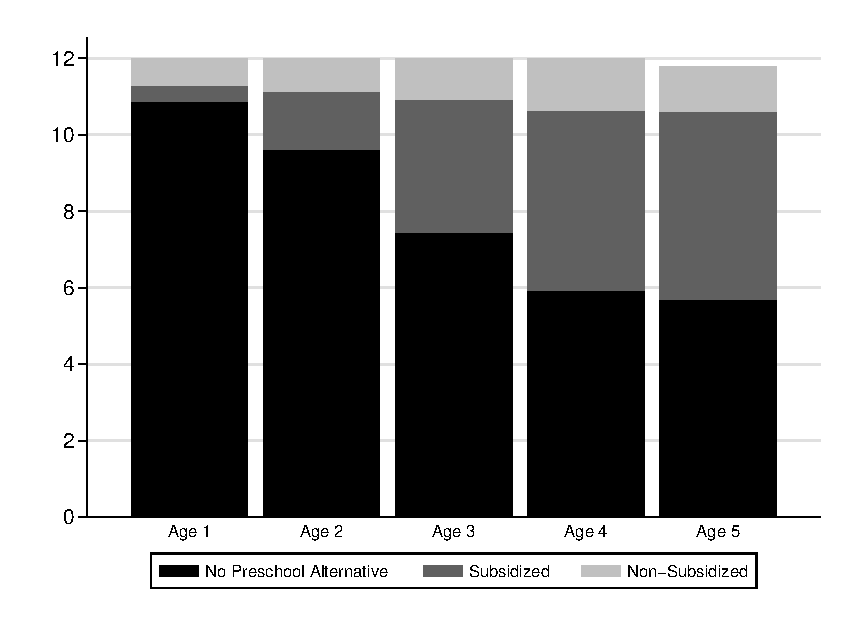
\includegraphics[width=18em]{output/blackwhite_CCnumber_care}
\end{figure}
\hyperlink{substitution}{\beamerreturnbutton{Back}}
\end{frame}

%% ---------------------------------------------------------------------------

\begin{frame}
\frametitle{Treatment Effects before Control Substitution, Females}
\begin{center}
\begin{table}
	\caption{Treatment Effects, Females} \label{tab:onsetsfemales}
	\scalebox{.60}{ \begin{tabular}{cccccccccc}
  \toprule
      \scriptsize{Variable} & \scriptsize{Age} & \scriptsize{(1)} & \scriptsize{(2)} & \scriptsize{(3)} & \scriptsize{(4)} & \scriptsize{(5)} & \scriptsize{(6)} & \scriptsize{(7)} & \scriptsize{(8)} \\ 
    \midrule  

  \mc{1}{l}{\scriptsize{Std. IQ Test}} & \mc{1}{c}{\scriptsize{2}} & \mc{1}{c}{\scriptsize{10.700}} & \mc{1}{c}{\scriptsize{9.200}} & \mc{1}{c}{\scriptsize{13.950}} & \mc{1}{c}{\scriptsize{16.963}} & \mc{1}{c}{\scriptsize{13.910}} & \mc{1}{c}{\scriptsize{9.431}} & \mc{1}{c}{\scriptsize{6.680}} & \mc{1}{c}{\scriptsize{9.341}} \\  

     &  & \mc{1}{c}{\scriptsize{\textbf{(0.000)}}} & \mc{1}{c}{\scriptsize{\textbf{(0.000)}}} & \mc{1}{c}{\scriptsize{\textbf{(0.000)}}} & \mc{1}{c}{\scriptsize{\textbf{(0.000)}}} & \mc{1}{c}{\scriptsize{\textbf{(0.000)}}} & \mc{1}{c}{\scriptsize{\textbf{(0.000)}}} & \mc{1}{c}{\scriptsize{\textbf{(0.013)}}} & \mc{1}{c}{\scriptsize{\textbf{(0.000)}}} \\  

     & \mc{1}{c}{\scriptsize{3}} & \mc{1}{c}{\scriptsize{13.333}} & \mc{1}{c}{\scriptsize{12.563}} & \mc{1}{c}{\scriptsize{23.729}} & \mc{1}{c}{\scriptsize{29.326}} & \mc{1}{c}{\scriptsize{24.246}} & \mc{1}{c}{\scriptsize{9.211}} & \mc{1}{c}{\scriptsize{7.275}} & \mc{1}{c}{\scriptsize{9.177}} \\  

     &  & \mc{1}{c}{\scriptsize{\textbf{(0.000)}}} & \mc{1}{c}{\scriptsize{\textbf{(0.000)}}} & \mc{1}{c}{\scriptsize{\textbf{(0.000)}}} & \mc{1}{c}{\scriptsize{\textbf{(0.000)}}} & \mc{1}{c}{\scriptsize{\textbf{(0.000)}}} & \mc{1}{c}{\scriptsize{\textbf{(0.000)}}} & \mc{1}{c}{\scriptsize{\textbf{(0.039)}}} & \mc{1}{c}{\scriptsize{\textbf{(0.013)}}} \\ 
     \midrule
         \mc{1}{l}{\scriptsize{HOME Score}} & \mc{1}{c}{\scriptsize{0.5}} & \mc{1}{c}{\scriptsize{1.581}} & \mc{1}{c}{\scriptsize{0.749}} & \mc{1}{c}{\scriptsize{1.684}} & \mc{1}{c}{\scriptsize{1.131}} & \mc{1}{c}{\scriptsize{1.067}} & \mc{1}{c}{\scriptsize{0.980}} & \mc{1}{c}{\scriptsize{0.498}} & \mc{1}{c}{\scriptsize{0.438}} \\  

     &  & \mc{1}{c}{\scriptsize{\textbf{(0.039)}}} & \mc{1}{c}{\scriptsize{(0.250)}} & \mc{1}{c}{\scriptsize{(0.158)}} & \mc{1}{c}{\scriptsize{(0.250)}} & \mc{1}{c}{\scriptsize{(0.316)}} & \mc{1}{c}{\scriptsize{(0.224)}} & \mc{1}{c}{\scriptsize{(0.342)}} & \mc{1}{c}{\scriptsize{(0.316)}} \\  

     & \mc{1}{c}{\scriptsize{1.5}} & \mc{1}{c}{\scriptsize{2.668}} & \mc{1}{c}{\scriptsize{1.723}} & \mc{1}{c}{\scriptsize{4.729}} & \mc{1}{c}{\scriptsize{3.279}} & \mc{1}{c}{\scriptsize{4.661}} & \mc{1}{c}{\scriptsize{1.544}} & \mc{1}{c}{\scriptsize{0.992}} & \mc{1}{c}{\scriptsize{1.746}} \\  

     &  & \mc{1}{c}{\scriptsize{\textbf{(0.013)}}} & \mc{1}{c}{\scriptsize{(0.158)}} & \mc{1}{c}{\scriptsize{\textbf{(0.013)}}} & \mc{1}{c}{\scriptsize{\textbf{(0.092)}}} & \mc{1}{c}{\scriptsize{\textbf{(0.013)}}} & \mc{1}{c}{\scriptsize{(0.132)}} & \mc{1}{c}{\scriptsize{(0.263)}} & \mc{1}{c}{\scriptsize{(0.105)}} \\  

     & \mc{1}{c}{\scriptsize{2.5}} & \mc{1}{c}{\scriptsize{0.762}} & \mc{1}{c}{\scriptsize{0.832}} & \mc{1}{c}{\scriptsize{4.434}} & \mc{1}{c}{\scriptsize{5.502}} & \mc{1}{c}{\scriptsize{4.637}} & \mc{1}{c}{\scriptsize{-0.899}} & \mc{1}{c}{\scriptsize{-0.932}} & \mc{1}{c}{\scriptsize{-0.256}} \\  

     &  & \mc{1}{c}{\scriptsize{(0.224)}} & \mc{1}{c}{\scriptsize{(0.237)}} & \mc{1}{c}{\scriptsize{\textbf{(0.000)}}} & \mc{1}{c}{\scriptsize{\textbf{(0.000)}}} & \mc{1}{c}{\scriptsize{\textbf{(0.000)}}} & \mc{1}{c}{\scriptsize{(0.737)}} & \mc{1}{c}{\scriptsize{(0.737)}} & \mc{1}{c}{\scriptsize{(0.566)}} \\ 
     \midrule  
      \mc{1}{l}{\scriptsize{Parental Income}} & \mc{1}{c}{\scriptsize{1.5}} & \mc{1}{c}{\scriptsize{4,516}} & \mc{1}{c}{\scriptsize{7,539}} & \mc{1}{c}{\scriptsize{5,105}} & \mc{1}{c}{\scriptsize{8,682}} & \mc{1}{c}{\scriptsize{9,681}} & \mc{1}{c}{\scriptsize{4,309}} & \mc{1}{c}{\scriptsize{7,091}} & \mc{1}{c}{\scriptsize{7,337}} \\  

     &  & \mc{1}{c}{\scriptsize{\textbf{(0.066)}}} & \mc{1}{c}{\scriptsize{\textbf{(0.013)}}} & \mc{1}{c}{\scriptsize{(0.158)}} & \mc{1}{c}{\scriptsize{\textbf{(0.079)}}} & \mc{1}{c}{\scriptsize{\textbf{(0.039)}}} & \mc{1}{c}{\scriptsize{(0.105)}} & \mc{1}{c}{\scriptsize{\textbf{(0.066)}}} & \mc{1}{c}{\scriptsize{\textbf{(0.000)}}} \\  

     & \mc{1}{c}{\scriptsize{2.5}} & \mc{1}{c}{\scriptsize{222}} & \mc{1}{c}{\scriptsize{400}} & \mc{1}{c}{\scriptsize{-3,712}} & \mc{1}{c}{\scriptsize{894}} & \mc{1}{c}{\scriptsize{1,769}} & \mc{1}{c}{\scriptsize{1,598}} & \mc{1}{c}{\scriptsize{894}} & \mc{1}{c}{\scriptsize{3,227}} \\  

     &  & \mc{1}{c}{\scriptsize{(0.474)}} & \mc{1}{c}{\scriptsize{(0.434)}} & \mc{1}{c}{\scriptsize{(0.697)}} & \mc{1}{c}{\scriptsize{(0.408)}} & \mc{1}{c}{\scriptsize{(0.408)}} & \mc{1}{c}{\scriptsize{(0.355)}} & \mc{1}{c}{\scriptsize{(0.382)}} & \mc{1}{c}{\scriptsize{(0.224)}} \\  
     \midrule
      \mc{1}{l}{\scriptsize{Mother Works}} & \mc{1}{c}{\scriptsize{2}} & \mc{1}{c}{\scriptsize{0.168}} & \mc{1}{c}{\scriptsize{0.124}} & \mc{1}{c}{\scriptsize{0.323}} & \mc{1}{c}{\scriptsize{0.292}} & \mc{1}{c}{\scriptsize{0.309}} & \mc{1}{c}{\scriptsize{0.101}} & \mc{1}{c}{\scriptsize{0.082}} & \mc{1}{c}{\scriptsize{0.096}} \\  

     &  & \mc{1}{c}{\scriptsize{\textbf{(0.026)}}} & \mc{1}{c}{\scriptsize{\textbf{(0.079)}}} & \mc{1}{c}{\scriptsize{\textbf{(0.079)}}} & \mc{1}{c}{\scriptsize{(0.145)}} & \mc{1}{c}{\scriptsize{\textbf{(0.079)}}} & \mc{1}{c}{\scriptsize{(0.145)}} & \mc{1}{c}{\scriptsize{(0.211)}} & \mc{1}{c}{\scriptsize{(0.171)}} \\  

     & \mc{1}{c}{\scriptsize{3}} & \mc{1}{c}{\scriptsize{0.087}} & \mc{1}{c}{\scriptsize{0.047}} & \mc{1}{c}{\scriptsize{0.177}} & \mc{1}{c}{\scriptsize{0.145}} & \mc{1}{c}{\scriptsize{0.160}} & \mc{1}{c}{\scriptsize{0.066}} & \mc{1}{c}{\scriptsize{0.021}} & \mc{1}{c}{\scriptsize{0.057}} \\  

     &  & \mc{1}{c}{\scriptsize{(0.237)}} & \mc{1}{c}{\scriptsize{(0.368)}} & \mc{1}{c}{\scriptsize{(0.158)}} & \mc{1}{c}{\scriptsize{(0.316)}} & \mc{1}{c}{\scriptsize{(0.184)}} & \mc{1}{c}{\scriptsize{(0.276)}} & \mc{1}{c}{\scriptsize{(0.461)}} & \mc{1}{c}{\scriptsize{(0.276)}} \\  
     \bottomrule
     \end{tabular}}
\end{table}
\end{center}
\end{frame}

%% ---------------------------------------------------------------------------

\begin{frame}
\frametitle{Treatment Effects before Control Substitution, Males}
\begin{center}
\begin{table}
	\caption{Treatment Effects, Males} \label{tab:onsetsmales}
	\scalebox{.60}{
 \begin{tabular}{cccc}
  \toprule
      \scriptsize{Variable} & \scriptsize{Age} & \scriptsize{(1)} & \scriptsize{(2)} \\ 
    \midrule  

\mc{1}{l}{\scriptsize{Std. IQ Test}} & \mc{1}{c}{\scriptsize{2}} & \mc{1}{c}{\scriptsize{9.528}} & \mc{1}{c}{\scriptsize{11.036}} \\  

     &  & \mc{1}{c}{\scriptsize{\textbf{(0.000)}}} & \mc{1}{c}{\scriptsize{\textbf{(0.000)}}} \\  

     & \mc{1}{c}{\scriptsize{3}} & \mc{1}{c}{\scriptsize{13.410}} & \mc{1}{c}{\scriptsize{14.873}} \\  

     &  & \mc{1}{c}{\scriptsize{\textbf{(0.000)}}} & \mc{1}{c}{\scriptsize{\textbf{(0.000)}}} \\  
     \midrule
         \mc{1}{l}{\scriptsize{HOME Score}} & \mc{1}{c}{\scriptsize{0.5}} & \mc{1}{c}{\scriptsize{0.372}} & \mc{1}{c}{\scriptsize{0.039}} \\  

     &  & \mc{1}{c}{\scriptsize{(0.316)}} & \mc{1}{c}{\scriptsize{(0.487)}} \\  

     & \mc{1}{c}{\scriptsize{1.5}} & \mc{1}{c}{\scriptsize{-0.500}} & \mc{1}{c}{\scriptsize{-0.874}} \\  

     &  & \mc{1}{c}{\scriptsize{(0.645)}} & \mc{1}{c}{\scriptsize{(0.750)}}  \\  

     & \mc{1}{c}{\scriptsize{2.5}} & \mc{1}{c}{\scriptsize{0.141}} & \mc{1}{c}{\scriptsize{0.886}} \\ 

     &  & \mc{1}{c}{\scriptsize{(0.474)}} & \mc{1}{c}{\scriptsize{(0.263)}} \\  
	\midrule
	 \mc{1}{l}{\scriptsize{Parental Income}} & \mc{1}{c}{\scriptsize{1.5}} & \mc{1}{c}{\scriptsize{330}} & \mc{1}{c}{\scriptsize{-97.199}}  \\  

     &  & \mc{1}{c}{\scriptsize{(0.408)}} & \mc{1}{c}{\scriptsize{(0.461)}} \\  

     & \mc{1}{c}{\scriptsize{2.5}} & \mc{1}{c}{\scriptsize{673}} & \mc{1}{c}{\scriptsize{-941}}  \\  

     &  & \mc{1}{c}{\scriptsize{(0.382)}} & \mc{1}{c}{\scriptsize{(0.645)}} \\  
     \midrule
      \mc{1}{l}{\scriptsize{Mother Works}} & \mc{1}{c}{\scriptsize{2}} & \mc{1}{c}{\scriptsize{0.056}} & \mc{1}{c}{\scriptsize{0.038}} \\  

     &  & \mc{1}{c}{\scriptsize{(0.289)}} & \mc{1}{c}{\scriptsize{(0.368)}} \\  

     & \mc{1}{c}{\scriptsize{3}} & \mc{1}{c}{\scriptsize{0.150}} & \mc{1}{c}{\scriptsize{0.125}}  \\  

     &  & \mc{1}{c}{\scriptsize{\textbf{(0.066)}}} & \mc{1}{c}{\scriptsize{(0.184)}}  \\ 
     \bottomrule
     \end{tabular}
    }
\end{table}
\end{center}
\end{frame}

%% ---------------------------------------------------------------------------

\begin{frame}
\frametitle{Yale Estimates}
\begin{figure}
\caption{CBA (Summary)}
	\includegraphics[width=.8\columnwidth]{output/yaleresults.pdf}
\end{figure}
\end{frame}

%% ---------------------------------------------------------------------------

\begin{frame}
\frametitle{Tuesday Estimates}
\begin{figure}
\caption{CBA (Summary)}
	\includegraphics[width=.8\columnwidth]{output/pantanotuesdayestimates.pdf}
\end{figure}
\end{frame}

%% ---------------------------------------------------------------------------

\begin{frame}
\frametitle{Current Estimates}
\begin{center}
\begin{table}
	\caption{CBA Summary}
	\scalebox{.60}{\begin{tabular}{l c c c c c c }
\toprule
	&	\mc{2}{c}{Females}					&	\mc{2}{c}{Males}					&	\mc{2}{c}{Pooled}					\\
		\cmidrule(lr){2-3}						\cmidrule(lr){4-5}						\cmidrule(lr){6-7}					
Estimate 	&	IRR	&	B/C	&	IRR	&	B/C	&	IRR	&	B/C	\\
\midrule

% INSERT summary_tex.xls FILE BELOW
% INSERT summary_tex.xls FILE BELOW
% INSERT summary_tex.xls FILE BELOW

Baseline	&	0.11 	&	3.52	&	\textbf{0.16} &	9.21 	&	\textbf{0.13}	&	\textbf{5.80}	\\
	&	(0.12)	&	(2.67)	&	(0.11)	&	(8.33)	&	(0.06)	&	(2.86)	\\
Relative to Staying at Home	&	-0.14	&	\textbf{4.95}	&	0.06	&	4.29	&	\textbf{0.10} &	5.18	\\
	&	(0.13)	&	(2.02)	&	(0.11)	&	(4.75)	&	(0.05)	&	(3.19)	\\
Relative to Alternative Preschools	&	0.09		&	2.88	&	\textbf{0.21}	&	\textbf{13.64}	&	\textbf{0.13}	&	\textbf{5.56}	\\
	&	(0.11)	&	(1.85)	&	(0.13)	&	(5.72)	&	(0.06)	&	(2.88)	\\

% INSERT summary_tex.xls FILE ABOVE
% INSERT summary_tex.xls FILE ABOVE
% INSERT summary_tex.xls FILE ABOVE

\bottomrule
\end{tabular}}
\end{table}
\end{center}
\end{frame}

%% ---------------------------------------------------------------------------

\begin{frame}
\frametitle{Current Estimates}
\begin{center}
\begin{table}
	\caption{CBA Summary}
	\scalebox{.40}{\begin{tabular}{l r r r r r r r r r}																			
\toprule																			
&       \mc{3}{c}{Females}      &       \mc{3}{c}{Males}        &       \mc{3}{c}{Pooled}       \\																			
\cmidrule(lr){2-4}      \cmidrule(lr){5-7}      \cmidrule(lr){8-10}																			
Removed Component       &       NPV     &       IRR     &       B/C     &       NPV     &       IRR     &       B/C     &       NPV     &       IRR     &       B/C     \\																			
\midrule																			
None	&		&	0.15	&	\textbf{3.38}	&		&	-.10	&	6.75	&		&	0.10	&	\textbf{4.75}	\\
	&		&	(0.11)	&	(1.59)	&		&	(0.11)	&	(6.22)	&		&	(0.10)	&	(2.04)	\\ \\
Parental Income	&	\textbf{158,017}	&	0.05	&	1.72	&	45,511	&	-.10	&	6.27	&	\textbf{74,718}	&	0.08	&	\textbf{3.96}	\\
	&	(43,586)	&	(0.05)	&	(1.49)	&	(45,289)	&	(0.10)	&	(6.10)	&	(25,250)	&	(0.07)	&	(2.05)	\\
Subject QALY	&	0	&	0.15	&	\textbf{3.38}	&	0	&	-.10	&	6.75	&	0	&	0.10	&	\textbf{4.75}	\\
	&	(0.00)	&	(0.11)	&	(1.59)	&	(0.00)	&	(0.11)	&	(6.22)	&	(0.00)	&	(0.10)	&	(2.04)	\\
Subject Labor Income	&	44,201	&	0.16	&	\textbf{2.92}	&	124,655	&	-.06	&	5.44	&	93,992	&	-.08	&	\textbf{3.76}	\\
	&	(151,724)	&	(0.10)	&	(0.78)	&	(639,086)	&	(0.10)	&	(4.72)	&	(119,314)	&	(0.09)	&	(1.72)	\\
Subject Transfer Income	&	-1,276	&	0.16	&	\textbf{3.40}	&	-2,318	&	-.10	&	6.78	&	6,255	&	0.10	&	\textbf{4.68}	\\
	&	(34,263)	&	(0.11)	&	(1.60)	&	(33,759)	&	(0.11)	&	(6.23)	&	(9,411)	&	(0.10)	&	(2.04)	\\
Medical Expenditures	&	14,344	&	0.15	&	\textbf{3.23}	&	14,905	&	\textbf{0.13}	&	6.59	&	14,645	&	\textbf{0.10}	&	\textbf{4.60}	\\
	&	(82,883)	&	(0.15)	&	(1.55)	&	(146,935)	&	(0.10)	&	(6.17)	&	(39,129)	&	(0.07)	&	(2.03)	\\
Control Contamination	&	\textbf{19,884}	&	\textbf{0.12}	&	\textbf{3.17}	&	\textbf{15,608}	&	-.10	&	6.59	&	\textbf{15,073}	&	0.09	&	\textbf{4.59}	\\
	&	(3,147)	&	(0.08)	&	(1.59)	&	(2,324)	&	(0.11)	&	(6.21)	&	(2,229)	&	(0.09)	&	(2.03)	\\
Education Costs	&	-47,183	&	0.16	&	\textbf{3.88}	&	15,340	&	-.10	&	6.59	&	-11,353	&	0.11	&	\textbf{4.87}	\\
	&	(14,395)	&	(0.11)	&	(1.58)	&	(13,222)	&	(0.11)	&	(6.23)	&	(11,316)	&	(0.10)	&	(2.06)	\\
Crime Costs	&	\textbf{133,116}	&	0.14	&	1.98	&	427,343	&	0.07	&	2.25	&	\textbf{257,780}	&	0.07	&	2.04	\\
	&	(44,756)	&	(0.10)	&	(1.47)	&	(447,081)	&	(0.09)	&	(3.64)	&	(172,485)	&	(0.06)	&	(1.15)	\\ \\
Deadweight Loss	&		&	0.23	&	\textbf{4.70}	&		&	-.10	&	9.70	&		&	0.13	&	\textbf{6.77}	\\
	&		&	(0.18)	&	(2.36)	&		&	(0.12)	&	(9.36)	&		&	(0.13)	&	(3.04)	\\
0\% Discount Rate	&		&		&	\textbf{7.10}	&		&		&	14.72	&		&		&	\textbf{11.89}	\\
	&		&		&	(4.66)	&		&		&	(15.56)	&		&		&	(5.21)	\\
5\% Discount Rate	&		&		&	\textbf{2.39}	&		&		&	4.29	&		&		&	\textbf{2.81}	\\
	&		&		&	(0.90)	&		&		&	(3.61)	&		&		&	(1.17)	\\
\bottomrule																			
\end{tabular}																			
}
\end{table}
\end{center}
\end{frame}

%% ---------------------------------------------------------------------------

\begin{frame}
\frametitle{IRR Females, Treatment vs. Control} 
\begin{figure}
	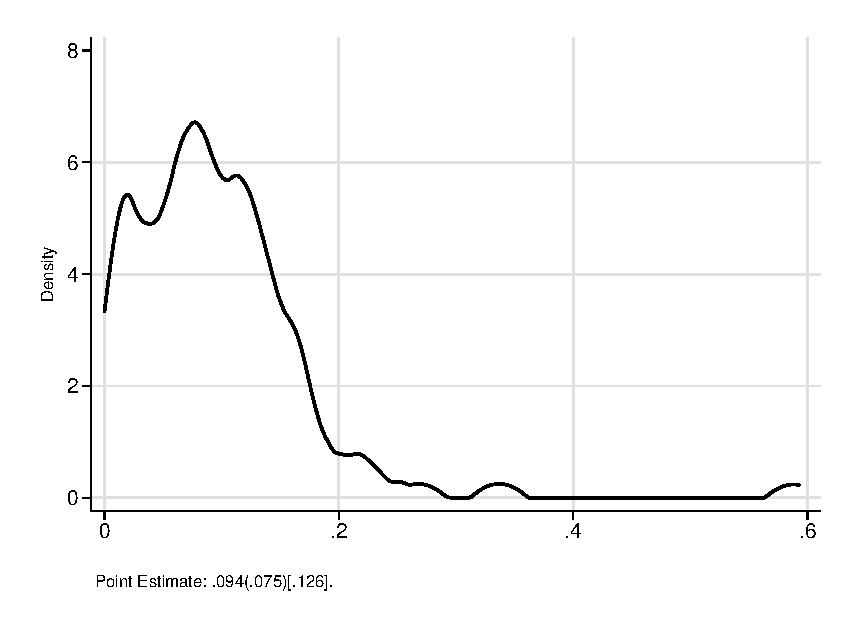
\includegraphics[width=.8\columnwidth]{output/irr_2_sexf.eps}
\end{figure}
\end{frame}

%% ---------------------------------------------------------------------------

\begin{frame}
\frametitle{IRR Males, Treatment vs. Control} 
\begin{figure}
	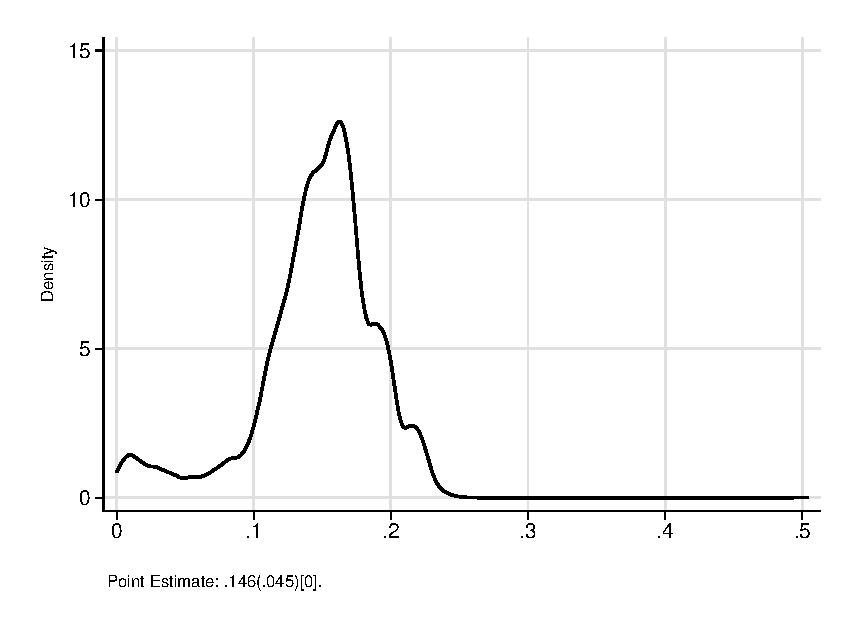
\includegraphics[width=.8\columnwidth]{output/irr_2_sexm.eps}
\end{figure}
\end{frame}

%% ---------------------------------------------------------------------------

\begin{frame}
\frametitle{IRR Pooled, Treatment vs. Control} 
\begin{figure}
	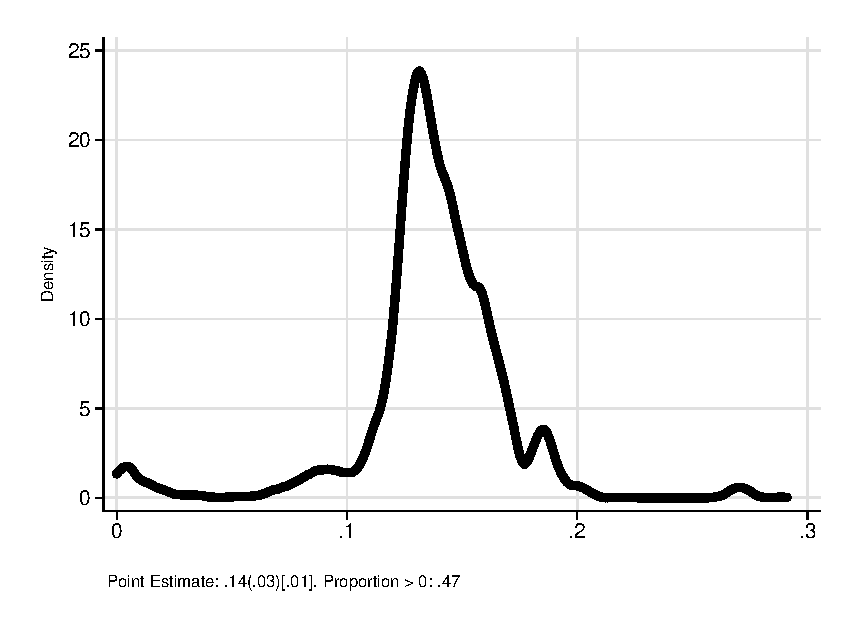
\includegraphics[width=.8\columnwidth]{output/irr_2_sexp.eps}
\end{figure}
\end{frame}

%% ---------------------------------------------------------------------------

\begin{frame}
\frametitle{IRR Females, Treatment vs. Control (Stay at Home)} 
\begin{figure}
	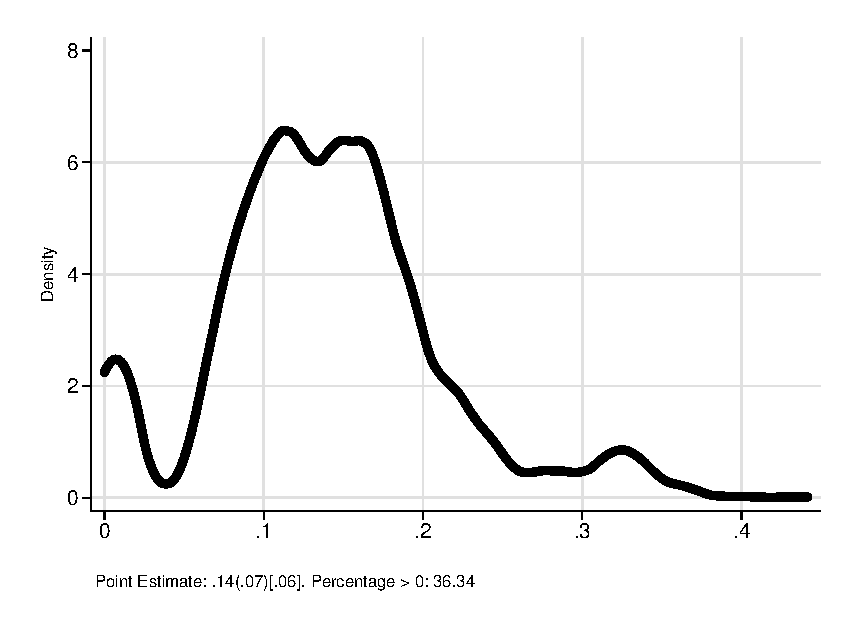
\includegraphics[width=.8\columnwidth]{output/irr_5_sexf.eps}
\end{figure}
\end{frame}

%% ---------------------------------------------------------------------------

\begin{frame}
\frametitle{IRR Males, Treatment vs. Control (Stay at Home)} 
\begin{figure}
	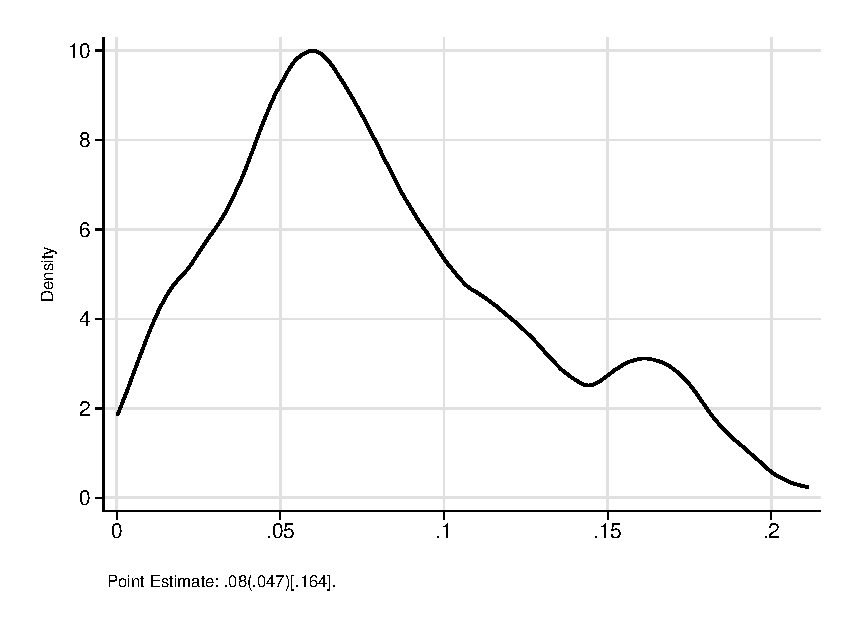
\includegraphics[width=.8\columnwidth]{output/irr_5_sexm.eps}
\end{figure}
\end{frame}

%% ---------------------------------------------------------------------------

\begin{frame}
\frametitle{IRR Pooled, Treatment vs. Control (Stay at Home)} 
\begin{figure}
	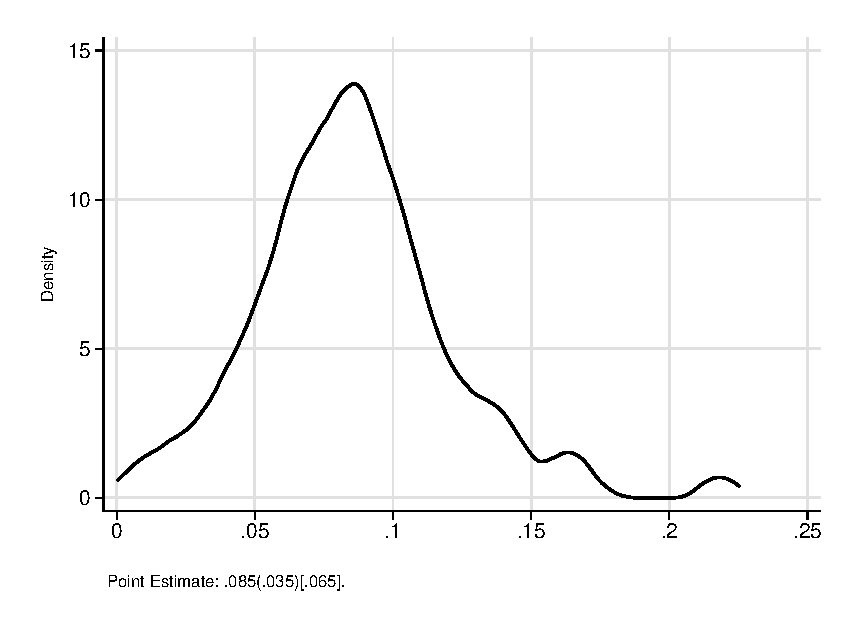
\includegraphics[width=.8\columnwidth]{output/irr_5_sexp.eps}
\end{figure}
\end{frame}

%% ---------------------------------------------------------------------------

\begin{frame}
\frametitle{IRR Females, Treatment vs. Control (Alternative Preschools)} 
\begin{figure}
	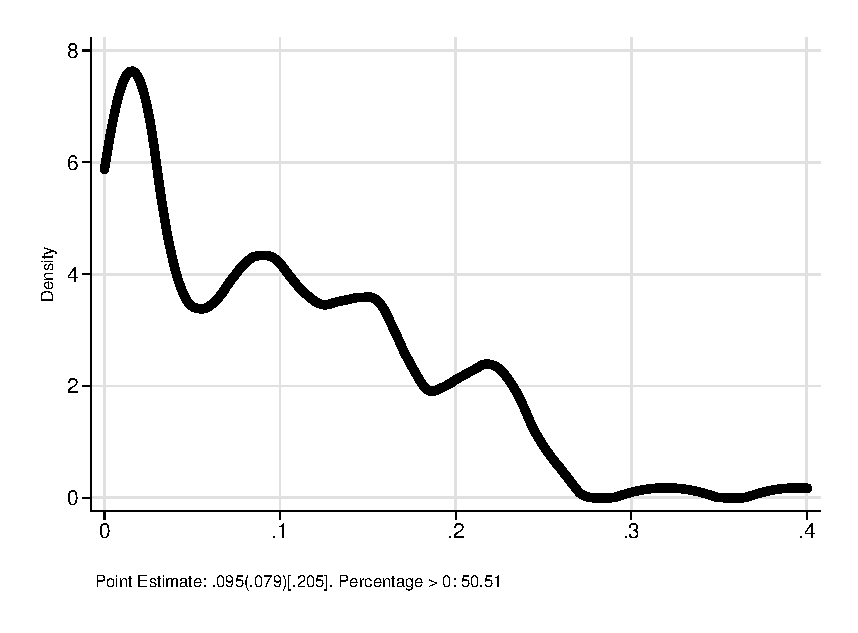
\includegraphics[width=.8\columnwidth]{output/irr_8_sexf.eps}
\end{figure}
\end{frame}

%% ---------------------------------------------------------------------------

\begin{frame}
\frametitle{IRR Males, Treatment vs. Control (Alternative Preschools)} 
\begin{figure}
	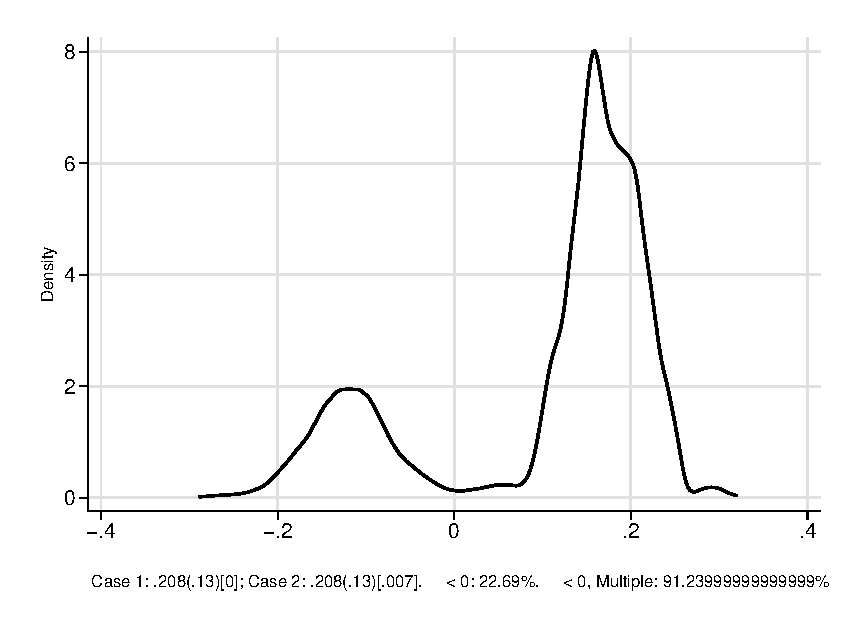
\includegraphics[width=.8\columnwidth]{output/irr_8_sexm.eps}
\end{figure}
\end{frame}

%% ---------------------------------------------------------------------------

\begin{frame}
\frametitle{IRR Pooled, Treatment vs. Control (Alternative Preschools)} 
\begin{figure}
	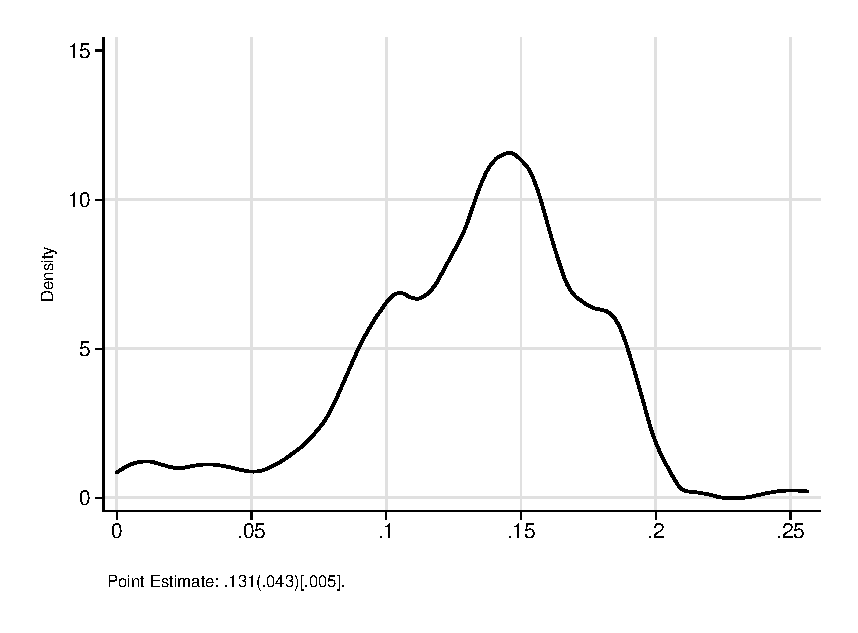
\includegraphics[width=.8\columnwidth]{output/irr_8_sexp.eps}
\end{figure}
\end{frame}

%% ---------------------------------------------------------------------------

\begin{frame}
\frametitle{B/C Females, Treatment vs. Control} 
\begin{figure}
	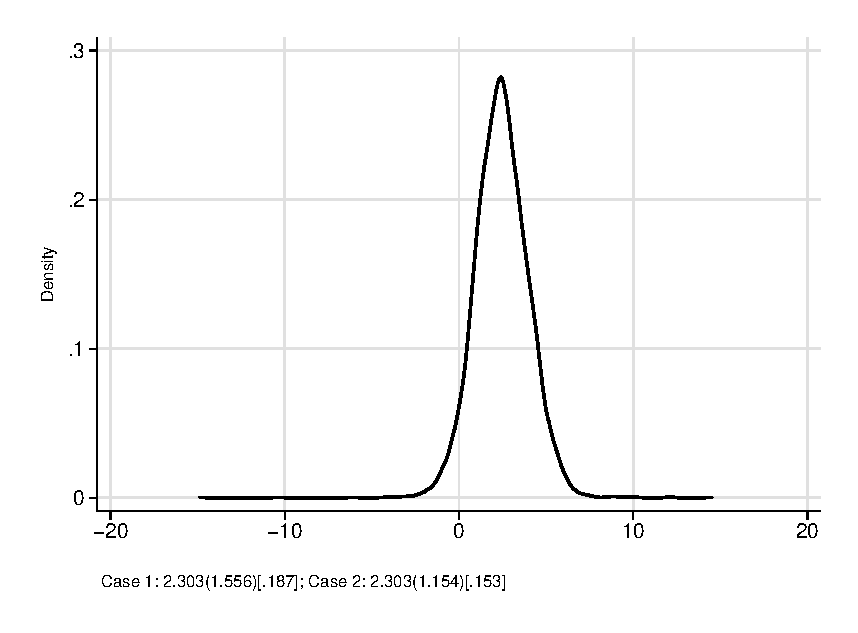
\includegraphics[width=.8\columnwidth]{output/ratios_2_sexf.eps}
\end{figure}
\end{frame}

%% ---------------------------------------------------------------------------

\begin{frame}
\frametitle{B/C Males, Treatment vs. Control} 
\begin{figure}
	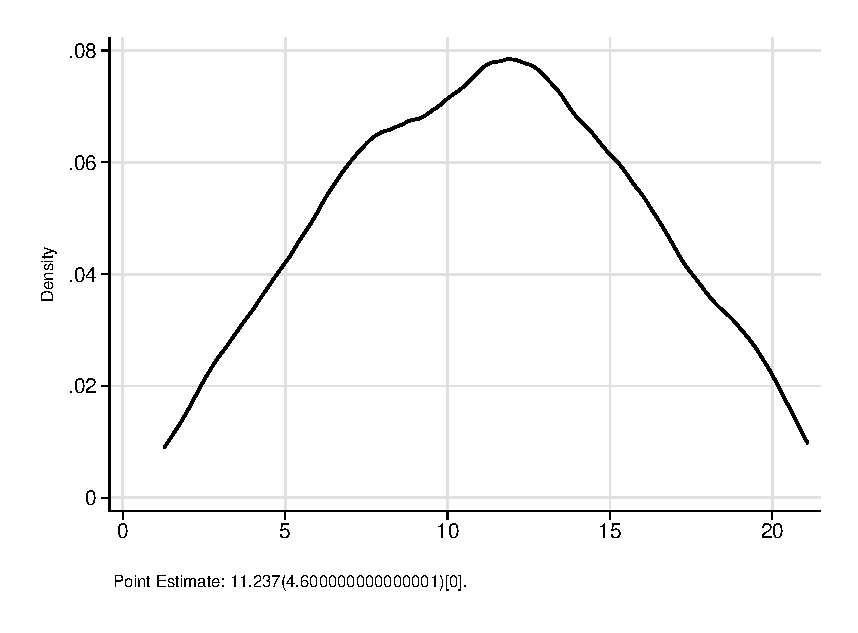
\includegraphics[width=.8\columnwidth]{output/ratios_2_sexm.eps}
\end{figure}
\end{frame}

%% ---------------------------------------------------------------------------

\begin{frame}
\frametitle{B/C Pooled, Treatment vs. Control} 
\begin{figure}
	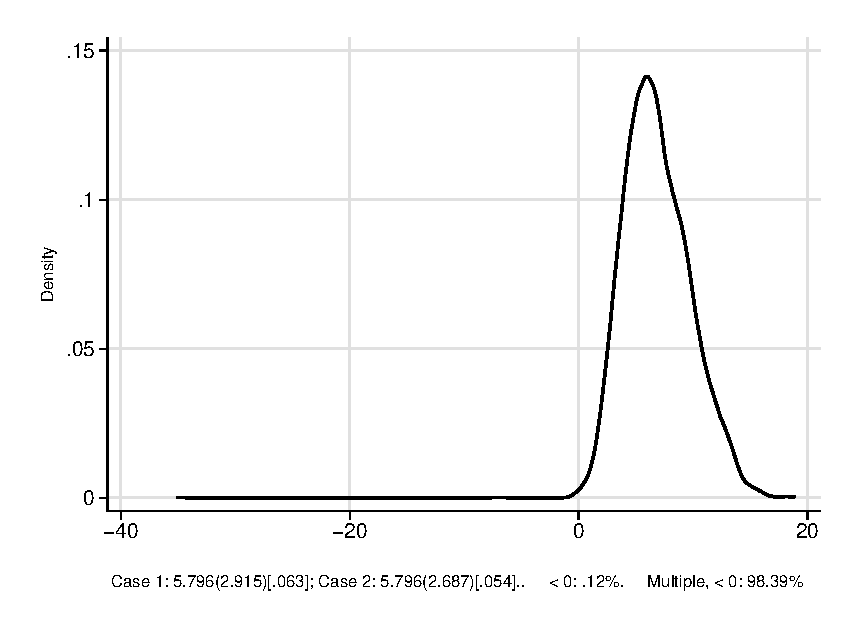
\includegraphics[width=.8\columnwidth]{output/ratios_2_sexp.eps}
\end{figure}
\end{frame}

%% ---------------------------------------------------------------------------

\begin{frame}
\frametitle{B/C Females, Treatment vs. Control (Stay at Home)} 
\begin{figure}
	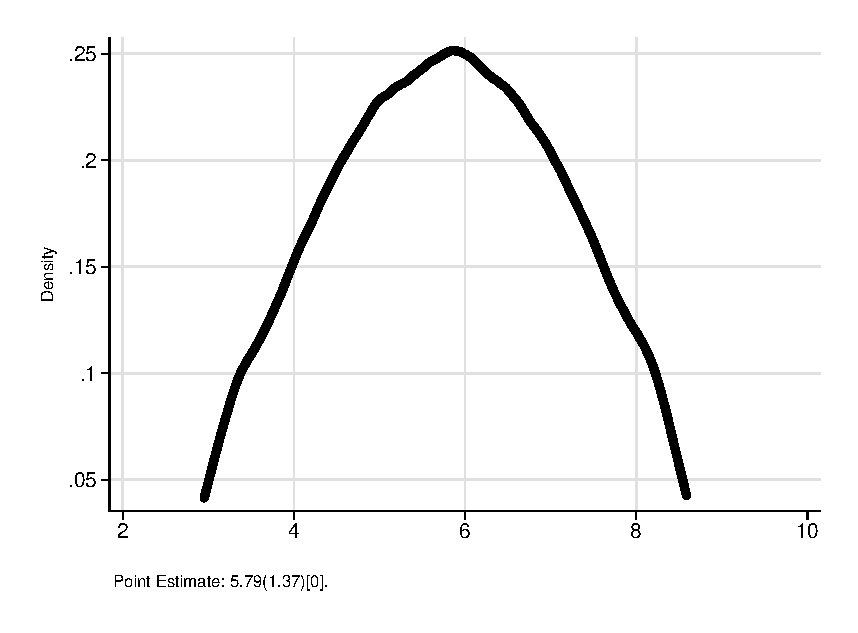
\includegraphics[width=.8\columnwidth]{output/ratios_5_sexf.eps}
\end{figure}
\end{frame}

%% ---------------------------------------------------------------------------

\begin{frame}
\frametitle{B/C Males, Treatment vs. Control (Stay at Home)} 
\begin{figure}
	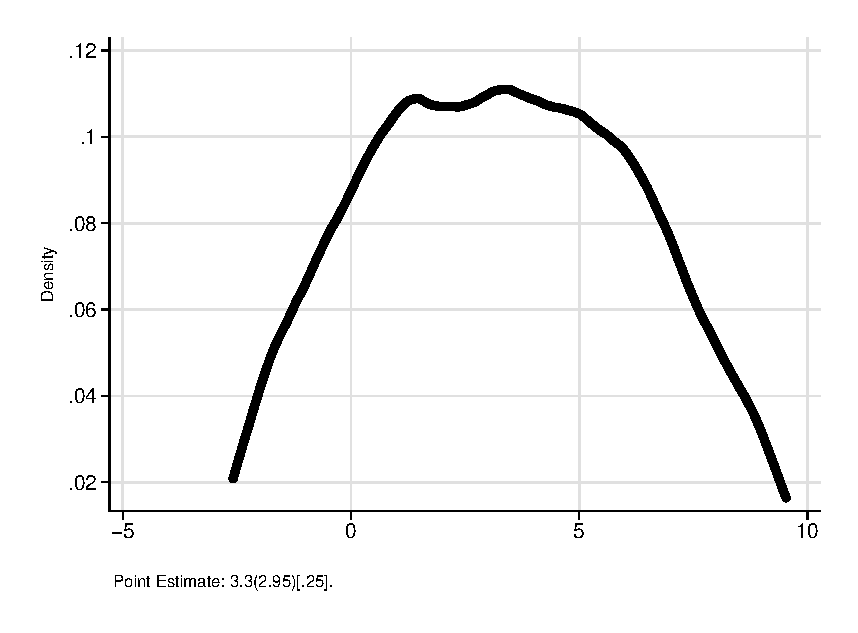
\includegraphics[width=.8\columnwidth]{output/ratios_5_sexm.eps}
\end{figure}
\end{frame}

%% ---------------------------------------------------------------------------

\begin{frame}
\frametitle{B/C Pooled, Treatment vs. Control (Stay at Home)} 
\begin{figure}
	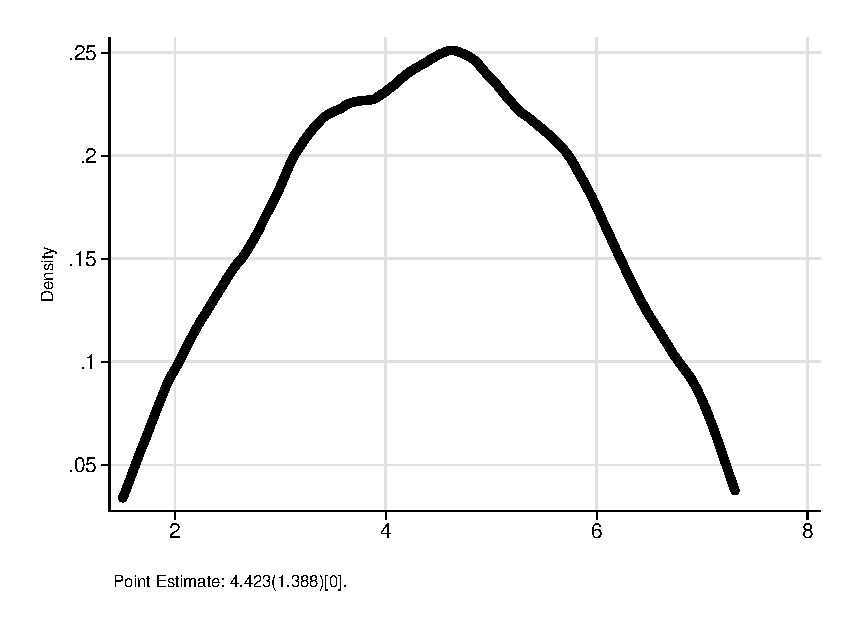
\includegraphics[width=.8\columnwidth]{output/ratios_5_sexp.eps}
\end{figure}
\end{frame}

%% ---------------------------------------------------------------------------

\begin{frame}
\frametitle{B/C Females, Treatment vs. Control (Alternative Preschools)} 
\begin{figure}
	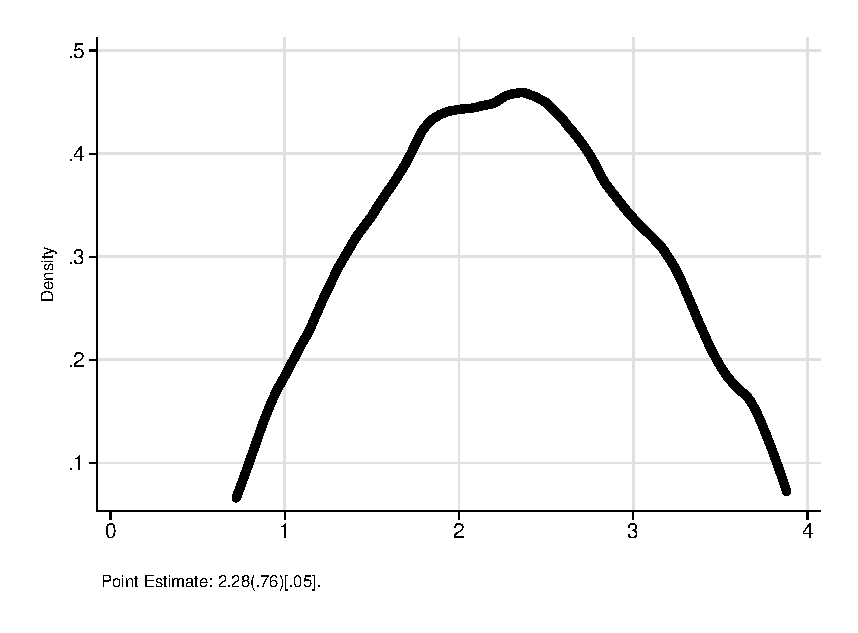
\includegraphics[width=.8\columnwidth]{output/ratios_8_sexf.eps}
\end{figure}
\end{frame}

%% ---------------------------------------------------------------------------

\begin{frame}
\frametitle{B/C Males, Treatment vs. Control (Alternative Preschools)} 
\begin{figure}
	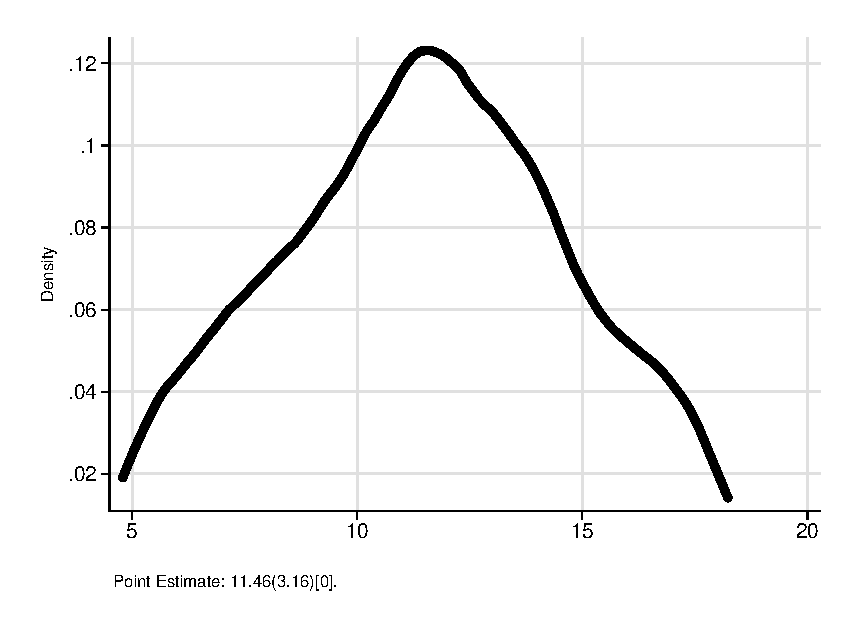
\includegraphics[width=.8\columnwidth]{output/ratios_8_sexm.eps}
\end{figure}
\end{frame}

%% ---------------------------------------------------------------------------

\begin{frame}
\frametitle{B/C Pooled, Treatment vs. Control (Alternative Preschools)} 
\begin{figure}
	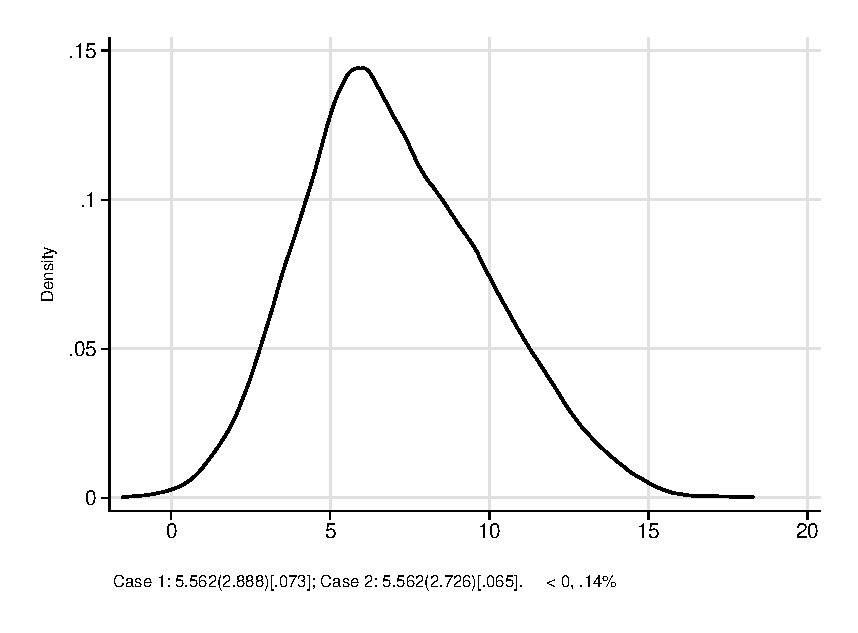
\includegraphics[width=.8\columnwidth]{output/ratios_8_sexp.eps}
\end{figure}
\end{frame}

%% ---------------------------------------------------------------------------

\begin{frame}
\frametitle{Current Estimates}
\begin{center}
\begin{table}
	\caption{CBA Summary}
	\scalebox{.60}{\begin{tabular}{l c c c c c c }
\toprule
	&	\mc{2}{c}{Females}					&	\mc{2}{c}{Males}					&	\mc{2}{c}{Pooled}					\\
		\cmidrule(lr){2-3}						\cmidrule(lr){4-5}						\cmidrule(lr){6-7}					
Estimate 	&	IRR	&	B/C	&	IRR	&	B/C	&	IRR	&	B/C	\\
\midrule

% INSERT summary_tex.xls FILE BELOW
% INSERT summary_tex.xls FILE BELOW
% INSERT summary_tex.xls FILE BELOW

Baseline	&	0.11 	&	3.52	&	\textbf{0.16} &	9.21 	&	\textbf{0.13}	&	\textbf{5.80}	\\
	&	(0.12)	&	(2.67)	&	(0.11)	&	(8.33)	&	(0.06)	&	(2.86)	\\
Relative to Staying at Home	&	-0.14	&	\textbf{4.95}	&	0.06	&	4.29	&	\textbf{0.10} &	5.18	\\
	&	(0.13)	&	(2.02)	&	(0.11)	&	(4.75)	&	(0.05)	&	(3.19)	\\
Relative to Alternative Preschools	&	0.09		&	2.88	&	\textbf{0.21}	&	\textbf{13.64}	&	\textbf{0.13}	&	\textbf{5.56}	\\
	&	(0.11)	&	(1.85)	&	(0.13)	&	(5.72)	&	(0.06)	&	(2.88)	\\

% INSERT summary_tex.xls FILE ABOVE
% INSERT summary_tex.xls FILE ABOVE
% INSERT summary_tex.xls FILE ABOVE

\bottomrule
\end{tabular}}
\end{table}
\end{center}
\end{frame}

%% ---------------------------------------------------------------------------

\begin{frame}
\frametitle{Current Estimates, Trimming}
\begin{center}
\begin{table}
	\caption{CBA Summary}
	\scalebox{.60}{\begin{tabular}{l c c c c c c }
\toprule
	&	\mc{2}{c}{Females}					&	\mc{2}{c}{Males}					&	\mc{2}{c}{Pooled}					\\
		\cmidrule(lr){2-3}						\cmidrule(lr){4-5}						\cmidrule(lr){6-7}					
Estimate 	&	IRR	&	B/C	&	IRR	&	B/C	&	IRR	&	B/C	\\
\midrule

% INSERT summary_tex.xls FILE BELOW
% INSERT summary_tex.xls FILE BELOW
% INSERT summary_tex.xls FILE BELOW

Baseline	&	0.09 	&	\textbf{2.53}	&	\textbf{0.14} &	\textbf{9.75} 	&	\textbf{0.13}	&	\textbf{5.56}	\\
	&	(0.05)	&	(0.97)	&	(0.05)	&	(4.64)	&	(0.05)	&	(2.39)	\\
Relative to Staying at Home	&	\textbf{0.13}	&	\textbf{4.77}	&	\textbf{0.08}	&	4.38	&	\textbf{0.10} &	\textbf{4.41}	\\
	&	(0.05)	&	(1.40)	&	(0.04)	&	(2.65)	&	(0.03)	&	(1.34)	\\
Relative to Alternative Preschools	&	0.09		&	\textbf{2.30}	&	\textbf{0.16}	&	\textbf{12.48}	&	\textbf{0.13}	&	\textbf{6.22}	\\
	&	(0.06)	&	(0.90)	&	(0.04)	&	(5.13)	&	(0.04)	&	(2.23)	\\

% INSERT summary_tex.xls FILE ABOVE
% INSERT summary_tex.xls FILE ABOVE
% INSERT summary_tex.xls FILE ABOVE

\bottomrule
\end{tabular}}
\end{table}
\end{center}
\end{frame}

%% ---------------------------------------------------------------------------

\begin{frame}
\frametitle{Current Estimates, No Controls}
\begin{center}
\begin{table}
	\caption{CBA Summary}
	\scalebox{.60}{\input{output/cba_summary_nocontrols_notrim}}
\end{table}
\end{center}
\end{frame}

%% ---------------------------------------------------------------------------

\begin{frame}
\frametitle{Current Estimates, Trimming and No Controls}
\begin{center}
\begin{table}
	\caption{CBA Summary}
	\scalebox{.60}{\begin{tabular}{l c c c c c c }
\toprule
	&	\mc{2}{c}{Females}					&	\mc{2}{c}{Males}					&	\mc{2}{c}{Pooled}					\\
		\cmidrule(lr){2-3}						\cmidrule(lr){4-5}						\cmidrule(lr){6-7}					
Estimate 	&	IRR	&	B/C	&	IRR	&	B/C	&	IRR	&	B/C	\\
\midrule

% INSERT summary_tex.xls FILE BELOW
% INSERT summary_tex.xls FILE BELOW
% INSERT summary_tex.xls FILE BELOW

Baseline	&	\textbf{0.10} 	&	3.08&	\textbf{0.17} &	\textbf{9.66} 	&	\textbf{0.11}	&	\textbf{4.89}	\\
	&	(0.06)	&	(2.22)	&	(0.11)	&	(4.72)	&	(0.07)	&	(2.64)	\\
Relative to Staying at Home	&	\textbf{0.13}	&	6.64	&	0.05	&	3.11	&	\textbf{0.11} &	6.59 	\\
	&	(0.09)	&	(4.63)	&	(0.11)	&	(4.46)	&	(0.06)	&	(4.47)	\\
Relative to Alternative Preschools	&	0.09		&	1.87	&	\textbf{0.20}	&	\textbf{13.98}	&	0.12	&	4.72	\\
	&	(0.08)	&	(2.02)	&	(0.13)	&	(5.72)	&	(0.09)	&	(3.04)	\\

% INSERT summary_tex.xls FILE ABOVE
% INSERT summary_tex.xls FILE ABOVE
% INSERT summary_tex.xls FILE ABOVE

\bottomrule
\end{tabular}}
\end{table}
\end{center}
\end{frame}
\clearpage

%% ---------------------------------------------------------------------------
%% ----------------------------Appendix slides-----------------------------------------------

\appendix

%% ---------------------------------------------------------------------------


%%
%%--------------------------- Content ends here ---------------------------------------------------
%%

% --------------------- Bibliography hidden with a save box ---------------------------------------
\mode<all>
\bibliographystyle{chicago}
\savebox\hiddenbib{\parbox{\textwidth}{\bibliography{heckman}}}

\end{document} 